
\documentclass[conference,compsoc]{IEEEtran}

\usepackage{graphicx}
\usepackage{textcomp}

\begin{document}

\title{Ceph Recovery Performance}


\author{\IEEEauthorblockN{Gustavo Rayos}
\IEEEauthorblockA{Computer Science\\
New Mexico State University\\
Las Cruces, NM 88003\\
Email: grayos@cs.nmsu.edu}
\and
\IEEEauthorblockN{Satyajayant Misra}
\IEEEauthorblockA{Professor of Computer Science at NMSU\\
New Mexico State University\\
Las Cruces, NM 88003\\
Email: misra@cs.nmsu.edu}}

\maketitle


\begin{abstract}
Object storage is a major area of study in the field of high performance computing (HPC). High capacity systems require data redundancy via redundant array of inexpensive disks, known as RAID, or erasure coding to protect against hardware failure. RAID cannot offer high redundancy in larger systems due to scaling issues, therefore the use of object storage with erasure coding is recommended \cite{wang_evaluation}. Many companies have implemented object storage, and have different ideologies on how object storage should be implemented. One of these companies is Red Hat and their Ceph object store, which we will be testing in this study. Ceph benefits from all of the features of object storage, but also has features that other object storage solutions do not. One of the claimed features of Ceph is that it is self healing, meaning that it will recover on it’s own from hardware failure \cite{self_healing_claim}. The performance of recovery after hardware failure is extremely important in these HPC systems, because these systems can only handle a certain amount of failure at a time and need time to recover. During this recovery time, if another hardware failure occurs, this can lead to data loss which is unwanted. In this paper we present a study that tests the recovery performance of Ceph. We show our findings of the legitimacy of Red Hat\textquotesingle s self healing Ceph claim, and show that Ceph is indeed self healing, but we advise careful monitoring at all times in order to keep the system running at the capacity at which it was designed to run.  
\end{abstract}


\IEEEpeerreviewmaketitle


\section{Introduction}

The use of data redundancy in high performance computing is extremely important, and allows for data restoration if hardware failure, such as a hard drive failure, were to occur. Systems can use RAID or erasure coding to achieve data redundancy, but the use of RAID in larger systems has scaling issues, therefore the use of object storage with erasure coding is required for these larger high performance systems \cite {weatherspoon2002erasure}. In addition to increased scaling capability, object storage and erasure coding is beneficial over hierarchical file systems and RAID because it has the ability to access data via internet protocols, use custom metadata, and is compatible with commodity hardware \cite{mesnier2003object}.

There are various object storage solutions that HPC systems can run. One of these system is Ceph. Ceph is an open source object store which has all the benefits of object storage, but also has some added capabilities that other object storage software companies, such as GlusterFS and Swift, do not have. Ceph is backed by Red Hat, which makes the claim that Ceph is “self healing, and is able to recover from a hardware failure with little intervention from it’s administrators”. This claim is very interesting and should be investigated due to the fact that recovery time is directly related to the increased probability of data loss. A short recovery time is desired in order to decrease the probability of data loss in these HPC systems. Ceph storage clusters are based upon Reliable Autonomic Distributed Object Storage (RADOS). RADOS is an open source object storage service and is an integral part of the Ceph distributed storage system \cite{weil_rados}. 

In this paper, we will explore Ceph's healing capabilities, and also evaluate the performance of recovery by Ceph after a hard drive failure. In Section 2, we will discuss some of the aspects of object storage which may affect the recovery performance of Ceph. Section 3 will discuss in detail our hardware and software environment in which we conducted our testing. Finally, Section 4 will discuss our evaluation and findings of the Ceph object store, and it’s performance in recovering from a hardware failure.  


\section{Background}
Our research is motivated by the desire to have the most stable and reliable file system possible, that minimizes the probability of any data loss at any time. High performance systems are running applications that can generate up to petabytes of data, and can take days, or even weeks to complete. Therefore, we do not want to lose any of the data gathered from these jobs. Ceph is a large software that has many configurations with many variables, such as replication size, K + M values for erasure coding, erasure code plugins, such as Jerasure and ISA, and placement group (PG) numbers. The following sections will describe what these configurations are and how these configurations can affect recovery performance in Ceph. These are the configurations we will be investigating in our testing.  

\subsection{Placement Group Numbers}
Ceph uses the concept of pools, which are defined as logical partitions for storing objects \cite{ceph_about_pools}. There are two types of pools in Ceph, replicated pools and erasure coded pools. Inside a pool, there are a number of placement groups (PGs). The Controlled Replication Under Scalable Hashing (CRUSH) algorithm maps PGs to object storage devices (OSDs) dynamically \cite{wang_evaluation}. By using placement groups, there is a middle layer between a client and the Ceph OSD daemons to limit the control a client has on where it can store the object on the cluster. That is the job of the CRUSH algorithm. CRUSH first maps each object to a placement group, and then it maps the placement group to one or more OSD daemons. Figure \ref{fig:Pools} shows a diagram of how Ceph uses pools and placement groups to map an object to the OSDs \cite{weil2006crush}. We can see that a client will write an object to a pool of the client's choice. The pool can be either a replicated pool or an erasure coded pool, and will be configured to have a certain amount of placement groups. Ceph will find an primary OSD to write the object to using CRUSH and will assign a PG to the object. It will then replicate the object and choose the best OSDs to replicate the object to. All of these steps are controlled by the CRUSH algorithm.  

\begin{figure}

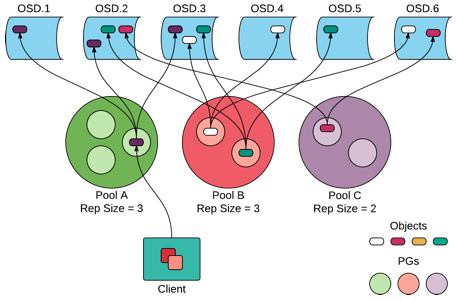
\includegraphics[width=\linewidth]{Pools.png}
\caption{Ceph uses pools and placement groups to find optimal location on OSDs.}
\label{fig:Pools}

\end{figure}

Placement group numbers may have an effect on Ceph recovery time. The larger the placement group number, the more placement groups there are on an OSD. This translates to if an OSD were to fail, then more PGs will have to be rebalanced into the other surviving OSDs. The more OSDs, the longer the recovery time. 

\subsection{Replication Size}
In replicated pools, we can set a value known as replication size. Replication size refers to how many copies of an object we want to store. This value is only tied to that particular pool in which the object is being written to. For instance, if we have a pool with replication size of 3, the first copy will be written to what is know as the primary OSD, then two subsequent copies will be written to two other OSDs in the cluster \cite{weil_high-performance}. 

Replication size may have an effect on recovery time based on how large the replication size value is. Replicated pools are known to require more raw storage than their corresponding erasure coded counterparts, so this may also lead to increased network traffic between nodes, in turn affecting recovery performance. 

\subsection{K + M Value}
Erasure coding is a method of protecting data by breaking the data object apart into fragments, expanded and encoded with redundant pieces, and storing those fragments across a set of multiple locations and storage devices. In Ceph, the erasure coding algorithm is run on the Object Storage Daemon (OSD) nodes. This algorithm can be resource heavy on the system, so proper Ceph configuration is desired in order to increase the overall performance of the cluster. One of the most important configurations in erasure coding is K + M value. 

The K variable represents the original amount of data chunks, and the M variable is the extra or redundant chunks that are added to provide protection from hardware failures. M also represents the number of OSDs that can fail without any data loss. Similar to replicated pools, the client writes an object to a pool of their choosing, then Ceph will pick a primary OSD to be the primary OSD and will assign a PG to the object. Then CRUSH will find secondary OSDs to write the K + M object chunks to. 

K + M values are used in erasure coding pools that defines how an object written to that pool will be fragmented and distributed among the OSDs. Figure \ref{fig:ErasureCoding} visually shows the erasure coding K + M values of 4 + 2 \cite{greenan2007disaster}. 

\begin{figure}

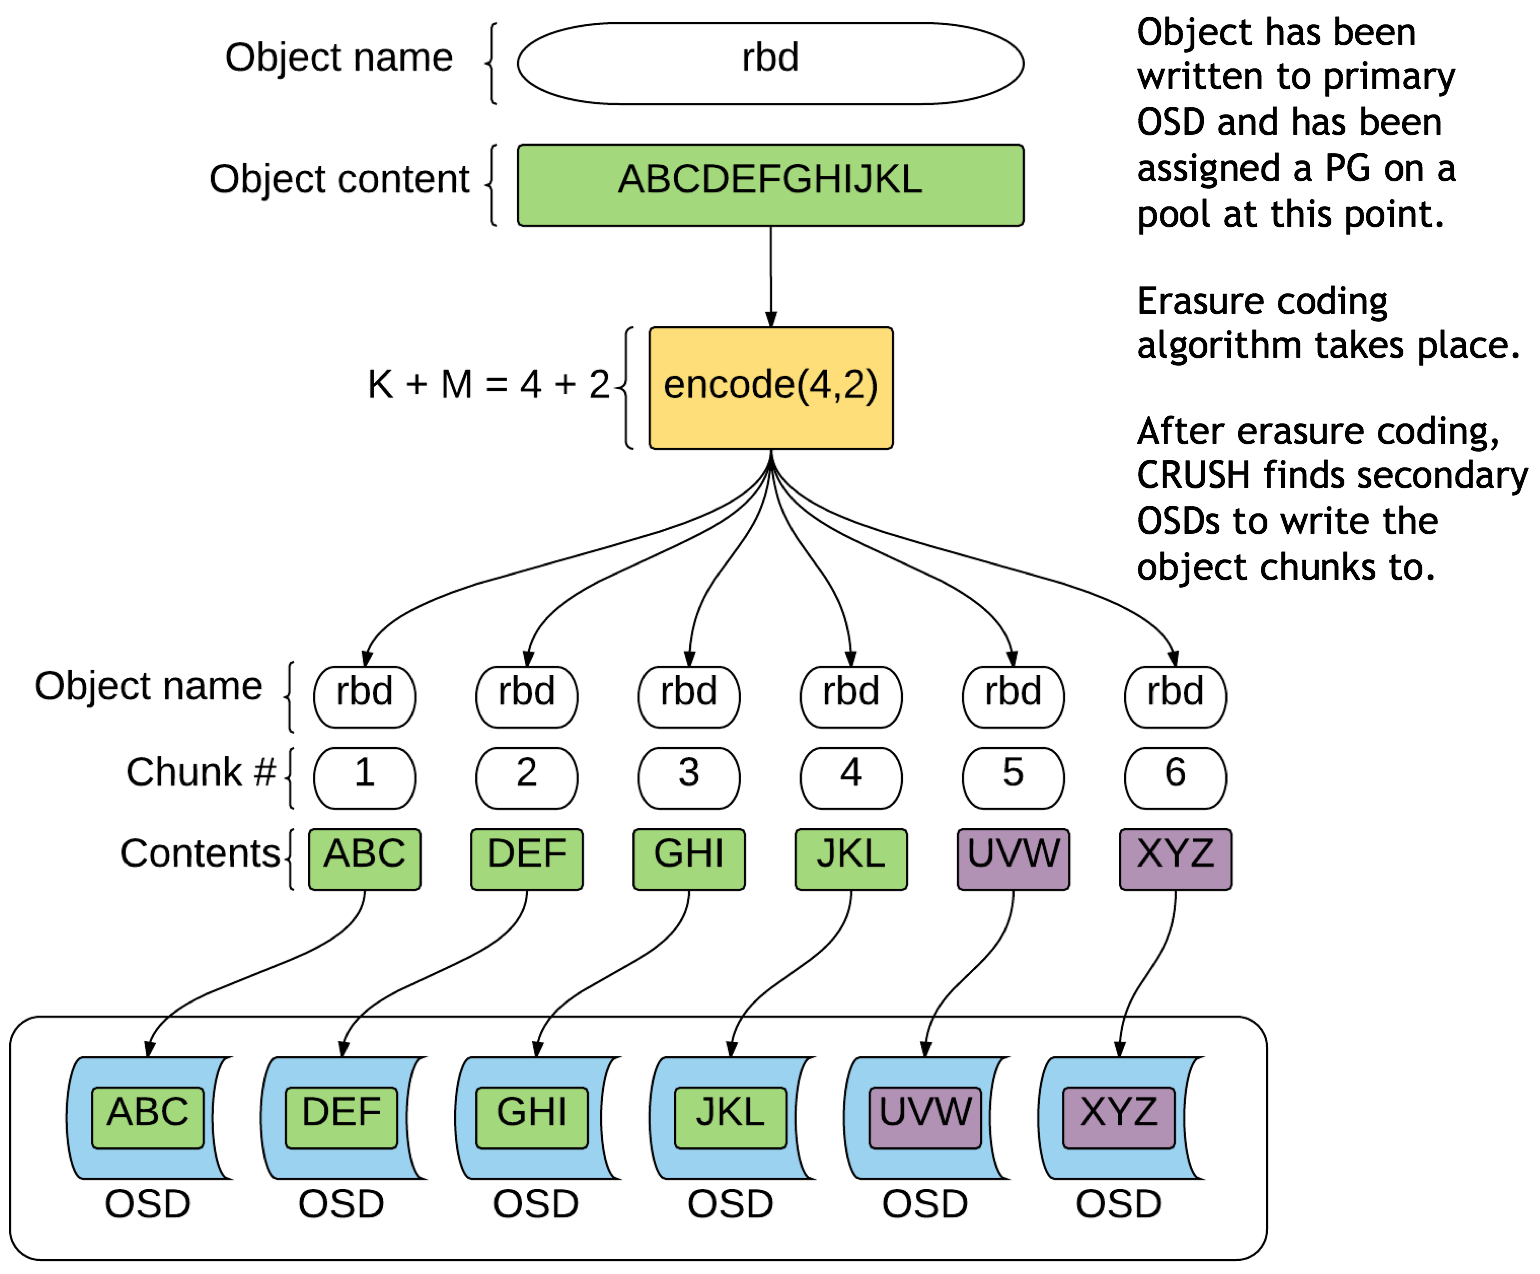
\includegraphics[width=\linewidth]{ErasureCoding.png}
\caption{Ceph uses K + M values for erasure coding.}
\label{fig:ErasureCoding}

\end{figure}

K + M values may have an affect in recovery time because erasure coding is very resource heavy. This may affect recovery time. Depending on how powerful the OSD nodes, this may have a direct impact on recovery performance if there is a CPU bottleneck on the OSDs. 

\subsection{Erasure Code Plugins}

In addition to K + M values, an erasure coded pool can also be configured with various erasure coding plugins. Two examples of these plugins are Jerasure and ISA \cite{erasure_coded_pools}. The jerasure plugin is the default plugin on Ceph and ISA is a plugin that was developed by Intel and is written in machine code to optimize the algorithm. Various other studies \cite{jerasure_vs_isa} suggest that ISA is indeed higher performance than jerasure, but have not studied the recovery performance of Ceph when using either jerasure or ISA \cite{erasure_coded_pools}. 

Different erasure code plugins may have different effects on Ceph\textquotesingle s recovery time because of the general performance of the plugin. 

\subsubsection{Jerasure Plugin}

The Jerasure plugin is the most generic and flexible erasure code plugin to use with Ceph, which is why it is the default plugin. The Jerasure plugin encapsulates the Jerasure library. It is able to run on most processors and is able to accept and apply all of the parameters of the Ceph erasure coding values. 

\subsubsection{ISA Plugin}

The ISA plugin encapsulates the ISA library and is only able to run on Intel processors. Other studies have demonstrated that while running Intel processors, ISA performs faster than the default Jerasure plugin \cite{jerasure_vs_isa}. Optimizations using some platform specific instructions enable ISA to perform better than the Jerasure plugin which is more generic and meant to be run on many platforms and processors \cite{isa}.

\section{System Environment}
Our test environment is made possible by NMC PRObE, which is a one of a kind computer facility dedicated to large scale systems research. Our cluster consists of twelve compute nodes running Ubuntu 14.04 on dual Quad Xeon E5504 CPUs clocked at 2.00 Ghz. Each node has 16 GiB of RAM and four 1 TB 5400 rpm HDDs are used as the OSDs for the Ceph storage. The nodes are interconnected with a gigabit interconnect at eth0, and a 10 gig interface at eth2. The Ceph object store consists of one monitor/admin node and eleven OSD nodes that are each running four OSD daemons. The monitor/admin node is responsible for monitoring the health of the Ceph cluster and for running commands remotely to all of the OSDs of the cluster. Figure \ref{fig:Environment} shows our testing environment.

\begin{figure}

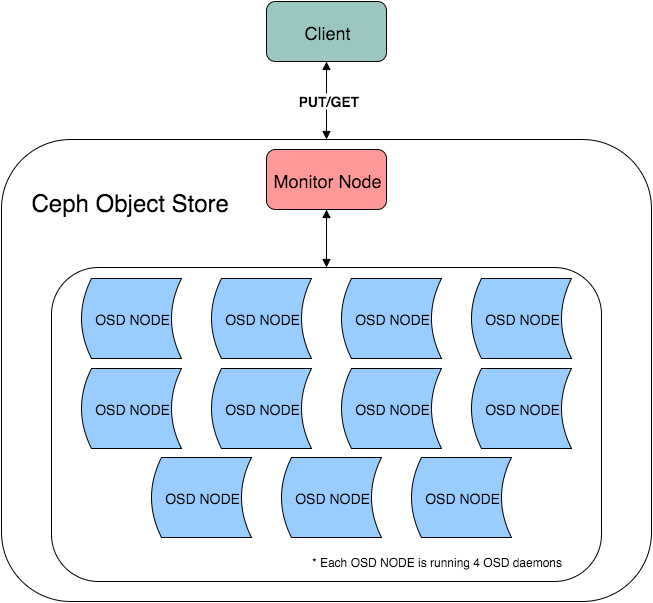
\includegraphics[width=\linewidth]{Environment.png}
\caption{Our test environment.}
\label{fig:Environment}

\end{figure}


\section{Recovery Performance Evaluation}

Our evaluation of Ceph recovery performance includes systematic testing of recovery as well as a real world approach to testing. We created multiple pool profiles in which we would test recovery performance. A total of 6 pool configurations were investigated. All pools were configured to have 512 PGs except for two. Pool 1 was configured to use the Jerasure plugin and was set with K + M values to 4 + 2. Pool 2 had the plugin set to ISA and had K + M values set to 4 + 2 as well. By doing this we were able to test the difference in plugin performance between the two. Pool 3 was set to use the Jerasure plugin and also had K + M = 4 + 2, but differed from Pool 1 in that it had 1024 PGs and not 512 PGs. The difference in PG number was meant to test the difference in performance varying PG values can have. Pool 4 is a Jerasure pool with K + M values set to 8 + 3. Pool 5 was a Jerasure pool with K + M values set to 6 + 2. The last pool, Pool 6, was a replicated pool with a replication size set to 3 and with 2048 PGs. All of the pools except for one had the placement group value set to 512. Figure \ref{fig:Configurations} shows the configurations of each pool. 

We first established a baseline for the write speed performance of each pool configuration by running a synthetic benchmarking tool called RADOS Bench, which was designed by Inktank specifically to benchmark a RADOS storage cluster \cite{wang_evaluation}. 

Also, to test the write performance, we will run a script that writes 100,000 one megabyte files to the Ceph object store, and time how long it takes to write the objects to the cluster. 

Once we have written the 100,000 objects to the 44 OSDs, we then test the recovery of a particular profile by simulating an OSD failure in the cluster, and timing how long it takes from when the drive fails, to when the Ceph monitor recognizes the Ceph object store as being in a ``Healthy'' state again. We repeat this process again simulating two OSDs as well.  

\subsection{Experimental Setup}

The experiments were performed on a Ceph cluster that was deployed using the built-in Ceph-deploy tools in Ceph. From the admin node of Ceph, we assigned a Ceph-monitor node, then the eleven Ceph-OSD nodes. The Ceph-OSD nodes were equiped with four 1Tb drives which we mounted and assigned OSD daemons to. After we obtained a healthy cluster, we were able to run the tests described in the previous paragraph. 

\begin{figure}

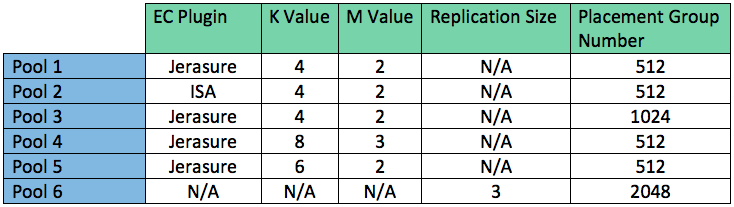
\includegraphics[width=\linewidth]{PoolConfigurations.png}
\caption{Pool configurations tested.}
\label{fig:Configurations}

\end{figure}

\subsubsection{Placement Group Number Determination}
The number of placement groups used were obtained by using the suggested formula in the Ceph documentation. To get the number of placement groups, we calculate (Number of OSDs * 100)/(OSD Per Object). OSD Per Object is the number of replicas in a replication pool, and for erasure coded pools, it is the sum of the K+M values \cite{maltzahn2010ceph}. For example, we have 44 OSDs and created an erasure coded pool of K + M = 4 + 2. We calculate (44 * 100)/6 = 733.33 placement groups. This number is rounded up or down to the nearest power of two. We used 512 placement groups.

\subsubsection{K + M Value Determination}

The K + M values of the pools were obtained by calculating the percentage of storage overhead the erasure coding will take up. For instance, if we have an erasure coded pool that is set to K = 4 and M = 2, that pool will use 6 OSD’s and will survive the loss of two OSDs. The overhead storage percentage is calculated by dividing M by K. In this case, K + M = 4 + 2, so the overhead is .5. In another pool set to K = 6 and M = 2, the overhead percentage will be .333 \cite{greenan2007disaster}.  

\subsection{Synthetic Write Benchmark}

The benchmark revealed that Intel\textquotesingle s ISA erasure code plugin is indeed faster than the default Jerasure plugin in terms of write speed. The jerasure 4+2 configuration is also a good performer as it came in second fastest out of all the configurations. The ISA pool configuration scored a result of 54.715 MB/sec while the jerasure profile scored 51.895 MB/sec. 

Changing placement group numbers also led to a change in write speed performance. Our jerasure pool with 1024 placement groups was the slowest of the erasure coded pools with an average write speed of 44.773 MB/sec.  The K + M = 8 + 3 pool performed adequately with a speed of 50.856 MB/sec. The 6 + 2 was slower than the 8 + 3 pools in terms of write performance with a speed of 49.066 MB/sec. The replicated pool had the slowest write speeds of all the pool configurations with a speed of 34.012 MB/sec. 

Figure \ref{fig:Synthetic} diagrams the synthetic write speed benchmark results of each pool configuration. 

\begin{figure}

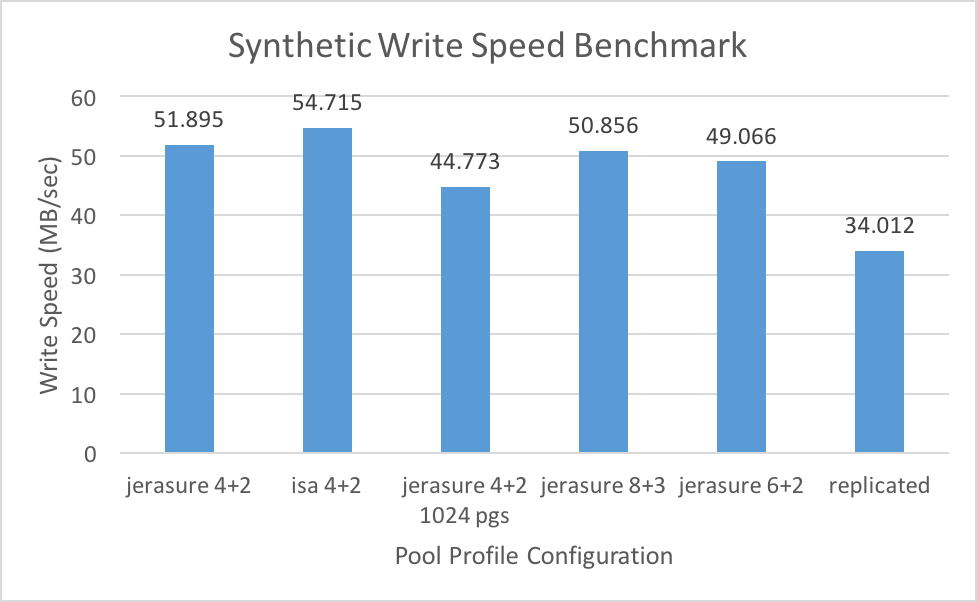
\includegraphics[width=\linewidth]{Synthetic.png}
\caption{Synthetic benchmark to test write performance.}
\label{fig:Synthetic}

\end{figure}
 
\subsection{Write 100,000 Objects Performance}

This test was designed to be a non-synthetic benchmark. The Jerasure and ISA plugins performed similarly in this test. Both plugins took roughly the same amount of time to write 100,000 objects to the cluster. For the jerasure 4+ 2 pool, it took 45.65 minutes, while the ISA 4 + 2 pool took 45.52 minutes. 

As we saw with the synthetic benchmarks, the 1024 placement group configuration showed slower write performance than the pools with less placement groups. This pool configuration took 52.55 minutes.The pool configurations with varying K + M values and 512 placement groups also performed faster than the 1024 placement group configuration. The jerasure 8 + 3 pool wrote the objects in 48.14 minutes, while the 6 + 2 pool wrote the objects in 48.68 minutes. The replicated pool configuration took the longest to write the 100,000 objects, taking 59.15 minutes. 

Figure \ref{fig:100,000} diagrams the write 100,000 objects performance. 

\begin{figure}

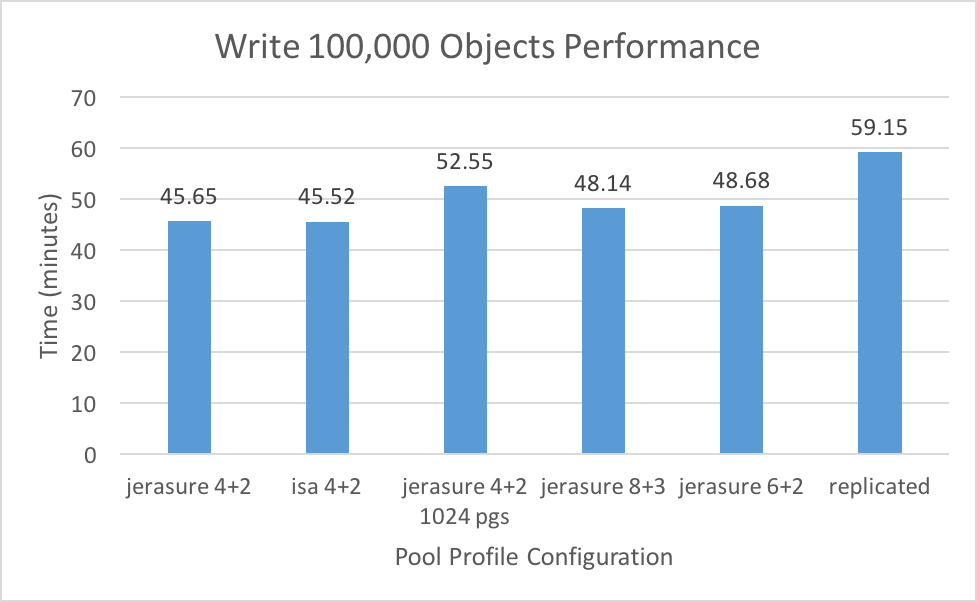
\includegraphics[width=\linewidth]{100,000.png}
\caption{Time to write 100,000 objects performance.}
\label{fig:100,000}

\end{figure}

\subsection{OSD Failure Recovery Time}

The previous write speed test performed allowed us to gather a baseline of each of the pool configurations. They also allowed us to fill the Ceph storage cluster with data in order to perform the OSD failure recover time benchmark. This benchmark is important it test the performance of Ceph being able to recover quickly. Quick recovey time is beneficial, because it decreases the chances of data loss by decreasing the time in which another OSD may fail, which may result in data loss. 

The jerasure and ISA plugins again performed similarly. The jerasure plugin configuration recovering from one OSD failure in 4.07 minutes and from two OSDs in 7.57 minutes. The ISA plugin recovered in 4.07 minutes for one OSD failure, and in 7.72 minutes for two OSD failures. 

The 1024 placement group configuration took 5 minutes to recover from one OSD, and took 8.28 minutes to recover from two OSD failures. Jerasure 8 + 3 was able to recover from one OSD failure in 9.55 minutes and in 11.23 minutes from two OSD failures. This pool is also able to recover from three OSD failures because of the M = 3 value, which was timed at 15.72 minutes. The pool configuration for K + M = 6 + 2 took 7.48 minutes to recover from one OSD failure, and 11.43 minutes for two OSD failures, which was the most time for two OSD recovery out of all of the pools. The replicated pool was the fastest at recovering from hardware failure. Recovering from one OSD failure took 2.23 minutes, and from two OSD failures took 3.78 minutes. 

Figure \ref{fig:Failure} diagrams the OSD failure recovery time of each pool configuration. 

\begin{figure}

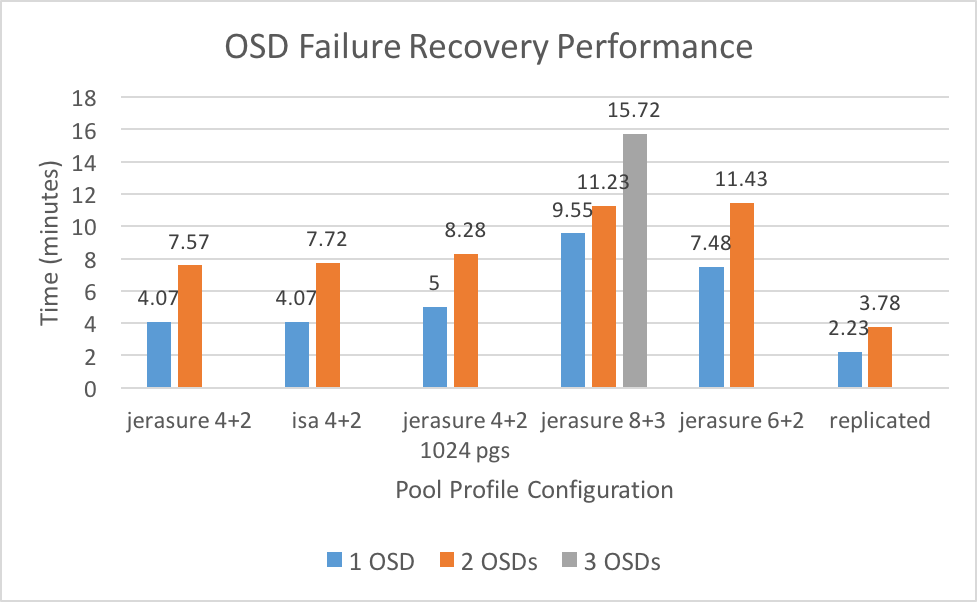
\includegraphics[width=\linewidth]{Failure.png}
\caption{Time to recover from OSD failure.}
\label{fig:Failure}

\end{figure}    

%Explain why?

Further investigation using Ganglia Cluster Monitoring software shows that CPU activity during erasure code recovery last longer than replicated pool recovery. In a replicated pool, when an OSD failure occurs, Ceph only needs to recognize the placement groups that have been effected and replicate the objects in those placement groups to new OSDs. In erasure coded pools, Ceph needs to recognize the PGs effected, run the erasure coding algorithm to recover the data using the parity chunks of the object, find new OSDs to write the recovered objects to, then finally run the erasure coding algorithm to create new data chunks and parity chunks for the object. The result of all of these erasure coding recover steps is sustained CPU activity, resulting in longer recovery time. 

Figures \ref{fig:ReplicationCpuReport} and \ref{fig:ErasureCpuReport} show the differences in CPU activity between an erasure coded pool and a replicated pool. 

\begin{figure}

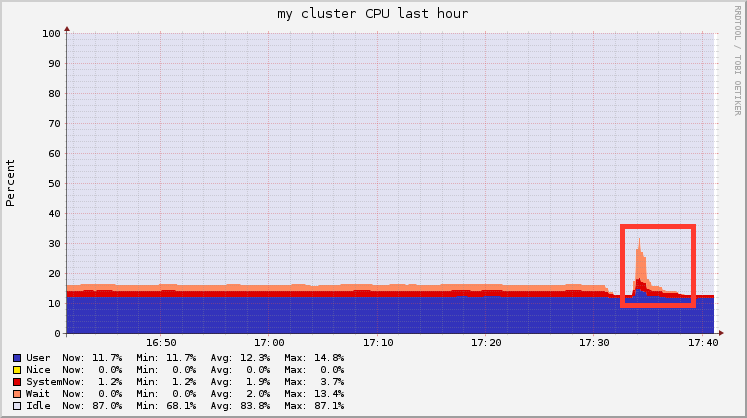
\includegraphics[width=\linewidth]{replication_cpu_report.png}
\caption{Replicated pool CPU activity.}
\label{fig:ReplicationCpuReport}

\end{figure}    

\begin{figure}

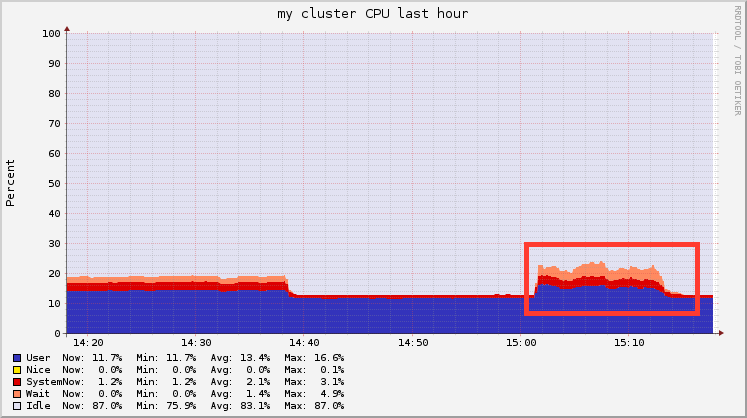
\includegraphics[width=\linewidth]{erasure_cpu_report.png}
\caption{Erasure coded pool CPU activity.}
\label{fig:ErasureCpuReport}

\end{figure}    

\subsection{Self-Healing Ceph}

The claim of Red Hat of Ceph being self-healing was tested as a result of testing OSD failure. When an OSD failed, Ceph was able to recover on it's own with little intervention from the Ceph administrators. The cluster recognized the OSD failure, recovered the missing data in the cluster using the erasure coding algorithm, and rebalanced the data, which lead to a healthy Ceph cluster. This shows sufficient evidence that Ceph is self healing. 

\section{Experimental Results}

The difference between erasure coded and replication pools leads to drastic differences in Ceph recovery time. We found that although the replicated pool performed the worst in terms of write speeds, it was the best performer in terms of recovery. This is a result of recovery not needing to perform the erasure coding when an OSD goes down. Replicated pools are a lot simpler than erasure coded pools, but have the worst overhead storage percentage of all pools. In the case of our replication pool, the replication size was 3, which lead to 300 GB of data on the cluster, even though there was only 100 GB of unique data.

The results also tell us that write performance does not directly relate to the recovery performance of Ceph. At this time, we would advise careful configuration when using erasure coding. Overhead storage percentage is an important consideration. The lower the overhead storage percentage, the lower the performance. Although the performance of the K + M = 8 + 3 configuration was the slowest, we would recommend these values as this pool was the only pool able to recover from 3 OSD failure while also having a low overhead storage percentage. Lowering the k value of this pool will lead to faster performance, but will increase the overhead storage performance. 

\section{Conclusions and Future Work}

In this study, we described the self healing ability of Ceph, and evaluated the performance of recovery after hard drive failure. We investigated the time it took from when an OSD were to fail, to when Ceph recognized itself as being healthy again. The various pool configurations Ceph uses definitely affects the recovery time of the cluster.

From the various tests we conducted, we conclude that the ISA plugin is simply more optimized than the default jerasure plugin as it is coded in assembly language. This results in the fastest recovery time out of all of the pool configurations. 

Placements groups also had a significant result on recovery time. Our pool configuration with 1024 placement groups took the longest to recovery of all erasure code profiles. We conclude that the increased number of placement groups resulted in the erasure coding algorithm having to sort through more placement groups. Therefore, the number of placement groups is directly related to the recovery time from hardware failure.  

K + M values are also very important to consider when creating a pool in Ceph. The storage overhead percentage can be calculated from these K + M values. 

\begin{itemize}
\item 4 + 2 = .5 Overhead Storage Percentage
\item 8 + 3 = .375 Overhead Storage Percentage
\item 6 + 2 = .333 Overhead Storage Percentage
\end{itemize}

From the tests performed, we can conclude that the overhead storage percentage is inversely related to the recovery performance of Ceph. 

To add to this investigation, we must further understand the Ceph software on a more underlying level. This will lead to both a better performance Ceph object store in terms of write and read performance, while also maintaining the reliability and scalability that Red Hat and the designers of Ceph intended.

Future work includes testing how Ceph handles data corruption within the hard drives, and monitoring network activity during recovery. 

We hope to one day continue our studies with Ceph, and in turn be able to better understand how to implement a reliable and performant Ceph object store. 

\section{Acknowledgements}

I would like to thank my advisor Dr. Satyajayant Misra, professor at New Mexico State University, for advising me through this project and for providing a better understanding of the research procedure that I used. 

This material is also supported in part by the National Science Foundation under awards CNS-1042537 and CNS-1042543 (PRObE) \cite{Gibson+:login13}. 

\bibliography{Ceph}
\bibliographystyle{plain}


\end{document}


